 \documentclass[a4paper,12pt]{book}

\usepackage{verbatim}
\usepackage{graphicx}

% use the style package defined for CIIT Dissertations
\usepackage{ciit-dissertation}

% use lipsum for dummy text
\usepackage{lipsum}

% Define the bib resource file which contains the citation definitions
\addbibresource{thesis.bib}


% Declare all of the data required to create the frontmatter (title pages, declarations .etc)
\title{An analysis of Modified Newtonian Dynamics as a candidate for solving the ``Missing Mass Problem''}

\author{Eraj Gulraiz}
\registrationnumber{CIIT/FA12-BPH-004/ISB}
\department{Physics}
\campus{Islamabad}
\degreetype{\undergraduate}
\program{BS Physics}
\dissertationtype{Thesis}
\session{Spring 2016}
\submissiondate{June 12, 2016}

\supervisor{Dr. Abid H. Mujtaba}
\supervisordesignation{Assistant Professor}

\hod{Dr. Sadia Manzoor}
\hoddesignation{Associate Professor}

\externalexaminer{}
\externalexaminerdesignation{}
\externalexaminerinstitution{}
\externalexamineraddress{}

\dedication{To My Dear Parents}
\acknowledgement{After all the struggles and hardwork of a complete year, now is the time that I pay my gratitude to the people responsible for making this possible for me. I would first acknowledge the dedication and continuous co-operation of my supervisor "Dr. Abid Mujtaba". Thank you sir, for your constant support. With your help and motivation I was able to choose the right direction and successfully complete my thesis. 

I am grateful to my Parents for making me a part of this institution, where i could finally get on the track of my ambitions. Last but not the least I would thank my friends for getting me through the tough times. 

Thank you!}
\abstract{The galactic motion reveals a discrepancy in the acceleration, that leads to the idea of the Missing Mass Problem. Study of rotation curves of the galaxies can give us a solution to this problem. In this research, the rotation curve of Andromeda Galaxy has been reproduced and optimized according to its observed rotation curve. }


\begin{document}

    \makefrontmatter        % Create all of the pages before the first chapter: title, dedication, ack, abstract, ToC, LoF .etc

    \chapter{Introduction}

Astronomy is the oldest of the natural sciences, the study of the celestial objects,their positions, and characteristics. Astrophysics is the application of the Laws of Physics to understand Astronomy. In early times Astronomy only comprised of the observations of the motion of visible celestial objects, but with the passage of time, questions about the nature of the universe started to originate. Early studies only considered the Solar system but with the discovery of telescope scientists realized that there is more to the universe than just that. Now, in the era of modern Astronomy, scientists have found many astounding phenomenon happening in outer space \cite{introduction}.
The following research includes a study of the motion of a spiral galaxy namely Andromeda. The analysis of the motion will be done by studying the rotation curve of the specified galaxy. I will develop a set of calculations including computational work, that will prove us that the solution of the Missing Mass Problem can be found without invoking Dark Matter.
The first chapter of this thesis introduces the basic concepts that are the basis of the following research.
((written with progress))

\section{Literature View}

\subsection{Evolution of the Universe}
 The origin and evolution of the Universe is proposed by the widely accepted Big Bang Theory, according to which the universe was created as a consequence of giant explosion of very dense and hot matter. After the explosion it started to expand and cool down, this cooling down resulted in the formation of elements and then in the formation of planets, stars, galaxies and various celestial objects \cite{evolution}.

\subsection{Missing Mass Problem}
When the scientists studied the motion of the objects in the Solar system they fell right into the realms of Newtonian laws of kinematics. There was no question in these Laws until the scientists studied the large scale structures such as galaxies or cluster of galaxies. This was first observed by Jan Hendrick Oort in 1932, when he noticed that stars in the solar neighborhood moved faster than expected. In 1939, Horace Babcock measured the rotation curve to Andromeda Galaxy which resulted in the increasing mass to luminosity ratio \cite{missing_mass}. Similarly, in 1959 Louise Volders demonstrated that the spiral galaxy M33 does not spin according to the Keplerian Dynamics \cite{mm}. The Rotation Curves give us the information of change in velocity as we move away from the center of a system. There were two conclusions drawn from such errors, that either our understanding of the Gravity is not quite right, in the case when we study large scale structures or there is some hidden matter that is providing enough force to these structures to move with certain accelerations.

\subsection{Dark Matter vs. MOND}
   In 1933 Fritz Zwicky invoke the dark matter as a solution to this mass discrepancy problem by studying eight Coma galaxies. He calculated mass to light ratios of these galaxy and concluded that 90 percent of the mass that had been responsible for the observed ratio, was missing \cite{dm_3}. The other method to find about missing mass was to study the rotational velocities of galaxies. And it was assumed that the stars in the galaxies will follow the Kepler's law like the planets in the solar system, i.e. their velocities will show a decline as moving through the radius. So it was assumed that there is some invisible matter affecting their motion. That matter was named as Dark Matter.
\cite{mond} \cite{dm_1} \cite{dm_2} The mass discrepancy observed in the stellar systems only happens when the acceleration of gravity falls below a fix value i.e.$a_{0}= 1.2x10^-8 cm/s^2$.\cite{mond_1} In 1983, Mordehai Milgrom proposed a modification in the Newtons Dynamics that explains many properties of galaxies without  the need of non baryonic dark matter. It is also effective in describing the dynamics of galaxies and galaxy clusters and within some approximations, gravitational lensing \cite{mond_2} \cite{mond_3}. MOND and Dark Matter give conceptually different but operationally equivalent description of cosmic phenomenon.

\section{Aims and objective}

\section{Work Plan}
 This research is based on the work of Milgrom for solving the Missing Mass Problem. It focuses on calculation of Milgrom's constant to create an expected rotation curve without the mass descrepancy.
(still to work)

      \chapter{Modified Newtonian Dynamics (MOND) [6]}

MOND is an algorithm that allows us the calculations of distribution of the effective gravitational force in astronomical objects from the distribution of baryonic matter with one additional fundamental parameter that has the dimensions od acceleration. This  is done by the determination of rotation curves of disk galaxies, and relating it with normal keplerian motion of the galaxies.

 It is a numeric way of calculating the missing mass or the factor that is causing a descrepancy in mass. It relates MOND acceleration 'a' to Newtonian acceleration $a_{N}$ by the following formula \begin{equation}
 a_{N}= a\mu(\frac{a}{a_{N}})
\end{equation}
where $a_{N} = 1.2×10-8  cms-2$  is a constant of physics.
The interpolation function $\mu (a/a0)$ shows asymptotic behaviour $\mu=1$ when $a>> a0$,  which retrieves the Newtonian expression in strong field regime. And for $a << a0$ with these assumptions gives us the following expression,
\begin{equation}
a= \sqrt{a_{N}a_{0}}= \frac{\sqrt{GMa_{0}}}{r}
\end{equation}
different functions are used for $\mu$, currently most used function is :
\begin{equation}
(\frac{a}{a_{0}}) = \frac{\frac{a}{a_{0}}}{\sqrt{1+(\frac{a}{a_{0}})^2}•}
\end{equation}
it works well for galactic rotation and solving for a, it gives
\begin{equation}
a= a_{N}(\frac{1}{2}+\frac{1}{2\sqrt{1+(\frac{2a_{0}}{a_{N}})^2}})^\frac{1}{2}
\end{equation}
the above expression allows us to calculate the MOND acceleration provided Newtonian gravity is known.

\section{Area of Study}
  MOND has been tested successfully on spiral galaxies, so for this research we choose our nearest spiral galaxy i.e. Andromeda Galaxy.(work it out)

\subsection{Andromeda Galaxy}
  Andromeda, M31 or NGC 224 is the nearest spiral galaxy to Milky Way.  (still to work)

\subsection{Distance to the Galaxy}

The stars and galaxies are far apart from Earth, these distances can vary from a few parsecs to kilo and mega parsecs. It is important to calculate the distances in order to determine further properties of these objects. There are different techniques to calculate distances, that astronomers have developed.
A few of them are listed below:

\subsection{Standard Candles[12]}
 Cepheid variable stars are used to as cosmic distance ladders to measure distances. Cepheid variable stars are a part of star cycle, formed when a giant red star is about to die. These stars expand and contract, changing their brightness from lighter to dimmer.  They change their brightness in regular intervals of 1 to 70 days. And the relation between the time interval and apparent magnitude gives us distances by the following equation:
 \begin{equation}
 d= 10^{\frac{(m-M+5)}{5}}
 \end{equation}
where \textbf{m} is the apparent magnitude and \textbf{M} is the absolute magnitude.

\subsection*{Binary Stars [13]}

Binary stars system is the one which have two stars orbiting around a center of mass, hence they are gravitationally bound to each other. Almost \textbf{85} percent of the stars are binary in nature. Gravity hold the system together, both stars orbit their centre of mass (CM). The orbital periods and distances of these system vary enormously.If the stars are the same masses, they are equally distant from CM, otherwise more massive star is closer to the CM. Binary stars are difficult to observe directly, because systems are too distant to resolve each star. Astronomers use their light curve ; how apparent brightness changes with time, to calculate the distances. Binary stars are classified to following categories.

\begin{enumerate}

\item\textbf{Visual Binaries}

Some binary systems are close to Earth and have a significantly large distances between each    other, so they can be visualized individually in a telescope. These systems are known as visual binaries.

\item {Spectroscopic Binaries }

Most binary systems are too far to be resolved by telescopes, so they are detected by the Doppler Shifts in their spectral lines. Such systems are spectroscopic binary system. The two stars appear to be moving towards and away from us. So the one moving towards us is blue shifted while the one moving away is red shifted.


\item \textbf{Astrometric Binaries}

The Binary stars sometimes are too far or two close. Sometimes it is hard to distinguish between the two stars in the system, such systems of binary stars are known as Astrometric binary stars \cite{astrometric_binaries}.
% [http://csep10.phys.utk.edu/astr162/lect/binaries/astrometric.html]

\item \textbf{Eclipsing Binaries}
% [http://www.physics.sfasu.edu/astro/ebstar/ebstar.html]

The type of variable stars, that appear as single point of light , but due to brightness variation and spectroscopic observations we say they are two stars in close orbit around each other and seem like they eclipse each other \cite{eclipsing_binaries}.

% [http://www.physics.sfasu.edu/astro/ebstar/ebstar.html]

These binary systems give the best estimates of distances. this system of binary stars have two luminous stars. The graph of brightness versus time is known as Light curve of eclipsing binaries. Time is expressed as phase, and the unit of phase is orbital period. The brightness is measured as magnitude of the stars.
\begin{figure}
\centering
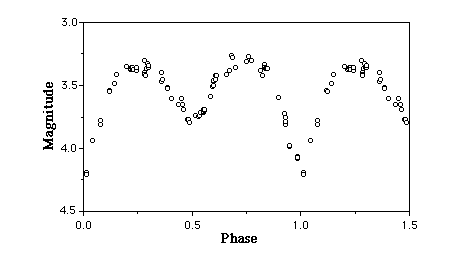
\includegraphics[scale=0.5]{LC}
\caption{Photometry of Beta Lyrae in 1992-1993}
\end{figure}

\end{enumerate}

\section*{Explanation of Light Curve}

The light curve is plotted as a consequence of the following movements of the stars in binary system.

\begin{itemize}
\item
If the stars are separated, we get lighy from both stars. Total amount of light will be indicated by the brightness on the brightness vs. time scale.
do it at home .. create figures and add phases of light curve. pages 5,6

\end{itemize}

\section{Computational Work}
The verification of Modiefied Newtonian Dynamics depends upon the Rotation Curve of the specific galaxy. The rotation curve gives us a relation between the rotational velocity and the distance of the astronomical object from teh centre. To gain the required result, I chose Andromeda Galaxy. Andromeda Galaxy is the nearest of our neighbours and its is a massive galaxy. To plot its rotation curve I was required to calculate the distances of the astronomical objects that comprise this galaxy and the mass distribution of the galaxy. Keeping the constraints of unavailability of any telescope in mind, i had to chose the technique of Image Analysis to relate the brightness to the mass distribution of the galaxy.
\subsection{Image Analysis of M31}
The image analysis is done by different techniques. It basically allows us to extract meaningful information from a digital image. There are different techniques that could be used for image analysis. Different programming languages are used for image analysis. I used Python language for this purpose. Python is a precise coding language, that allows us to write longer codes in a few lines.

The purpose of image analysis was to relate the luminous mass by using luminosity profile to the distance of each pixel from the centre. The following program was used for the whole process. The image used is just an image of a quadrant of the galaxy, and further calculations are done on the basis of an assumption of circular symmetry of the galaxy. Following is the image released by Hubble Telescope Images in $2015$ and is used for the analysis.
\begin{figure}[h!]
\centering
\includegraphics[scale=0.125]{andromeda.jpg}
\caption{Andromeda Galaxy, M31, NGC 224}
\end{figure}

\subsection{Program for Image Analysis}
The program was divided into a few parts to create a clear concept of purpose of each part. Following are the parts of the program.
\begin{enumerate}
\item \textbf{Defining the Image Dimensions}

The following code gives us the dimensions of the image being used and the spectral type of the image as the third entity.

\begin{verbatim}

andro = misc.imread('andromeda.jpg')
    (w, h,d) = andro.shape
\end{verbatim}

Output: (1918,6000,3)


\item \textbf{Calculation of the Distance of Certain Pixel from the Centre of the Galaxy}

This part defines the co-ordinates of the Origin as $x_{0}$ and $y_{0}$. This function iterates over the whole image to calaculate the distances of each pixel from the origin point by simple formula of the Pythagoras theorem.

\begin{verbatim}

x0 = 88.23
y0 =1675.78
def calc_distance(x0,y0,x,y):

    x_dist = (x - x0)
    y_dist = (y-y0)

    return  math.sqrt(x_dist*x_dist+y_dist*y_dist)

\end{verbatim}
Output:

\item \textbf{Intensity Calculation for Each Pixel}

The Intensity of each pixel is required to estimate the mass of each astronomiacal object in the galaxy, as intensity is directly proportional to the energy of the celestial object [1234].The image I used was an RGB image of the galaxy, to calculate the intensity of each pixel I had to convert it first into grayscale.This is done by fetching the RGB values of each pixel and taking square root of their squares divided by $3$. The pixel values are better to be normalized to get the results ranging from $0$ to $1$. The following part of the program explains this computation in a better way.

\begin{verbatim}

denom= math.sqrt(3)*255

def calc_gs_intensity(i):


    R = float(i[0])
    G = float(i[1])
    B = float(i[2])

    return math.sqrt(R*R+G*G+B*B)/denom


\end{verbatim}

Output:

\item \textbf{Storing the Data}

From the previously explained parts of the program, i got a large number of values. So, to use the calculated data it is necessary to create a data file, that can store maximum number of values and can again be used to plot a graph. The values from the distances and the intensity values are stored simultaneously in a single CSV (comma separated values) file.
\begin{verbatim}

with open('data.csv', 'w') as fout:

        for x in range(w):
            for y in range (h):

                r= calc_distance(x0,y0,x,y)
                i = calc_gs_intensity( andro[x,y] )

                print (r)
                print (i)

                fout.write(str(r) + "," + str(i)+ "\n")


\end{verbatim}
Output:

\item \textbf{Histogram}

Now, to analyze the mass distribution of M31, i plotted a histogram of radius versus Commulative Normalized Intensity. This gives us the mass density of the galaxy to be decreasing as we move far from the centre of the galaxy.
\begin{verbatim}
def main():

    reader = csv.reader (open('data.csv', 'rb'), delimiter=',')

    R = []
    I = []

    for row in reader:
        r= float(row[0])
        print r
        R.append( r )
        I.append( float(row[1]) )

    plt.hist(R, weights=I, bins = 100)
    plt.xlabel('radius   (pixels)    1kpc = 11.7px  ')
    plt.ylabel('Cummulative Normalized Intensity')
    plt.show()

\end{verbatim}

\begin{figure} [h]
\centering
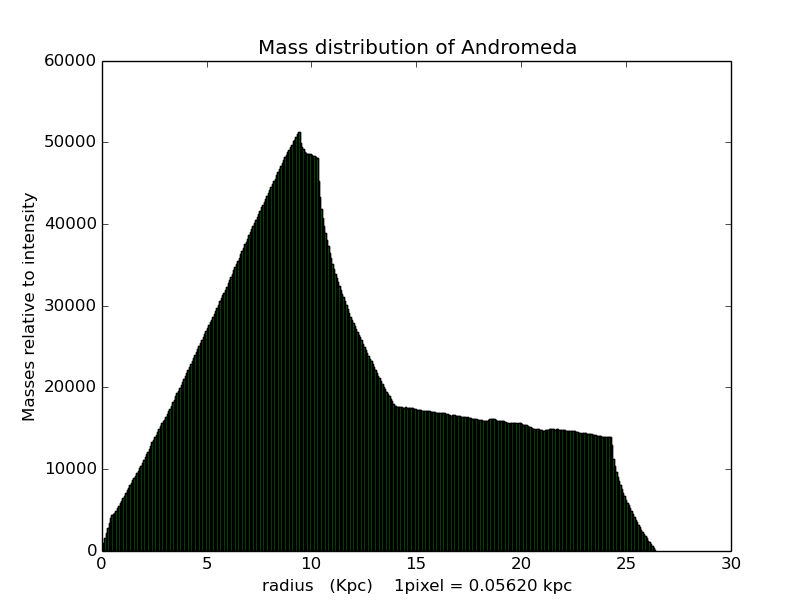
\includegraphics[scale=0.45]{400}
\caption{Mass Distribution of the Andromeda Galaxy }
\end{figure}

\end{enumerate}

\section{Calculation of Force}

According to Newton's second law, force is directly proportional to acceleration keeping mass constant. For the calculation of force on the objects inside the galaxy, we consider it to be a set of concentric rings. The histogram from the above section gives us the mass ditribution of the galaxy as moving through the radius. The force on a particle at radius 'r' will be the commulative effect of force due to the rings before and after the radius 'r'.

Let us consider the problem of finding the Gravitational potential in all space produced by a ring of mass M. In most analytical approaches to problem, solution is found only along the symmetry axis of the ring, where the integrals are expressed in terms of elementry functions. To solve for the potential of galaxy we require to calculate the off-axis solution that involves special functions or in this case Elliptic Integrals.
 
The system i am working on is given by the figure below. (figure 1 figure 2 )A ring of mass M and radius R, rests in xy axis with its centre at point O. A mass m is at a distance r as described in Figure (2.4), the 

\begin{figure}[!tbp] 
\centering
\begin{minipage}[b]{0.4\textwidth}
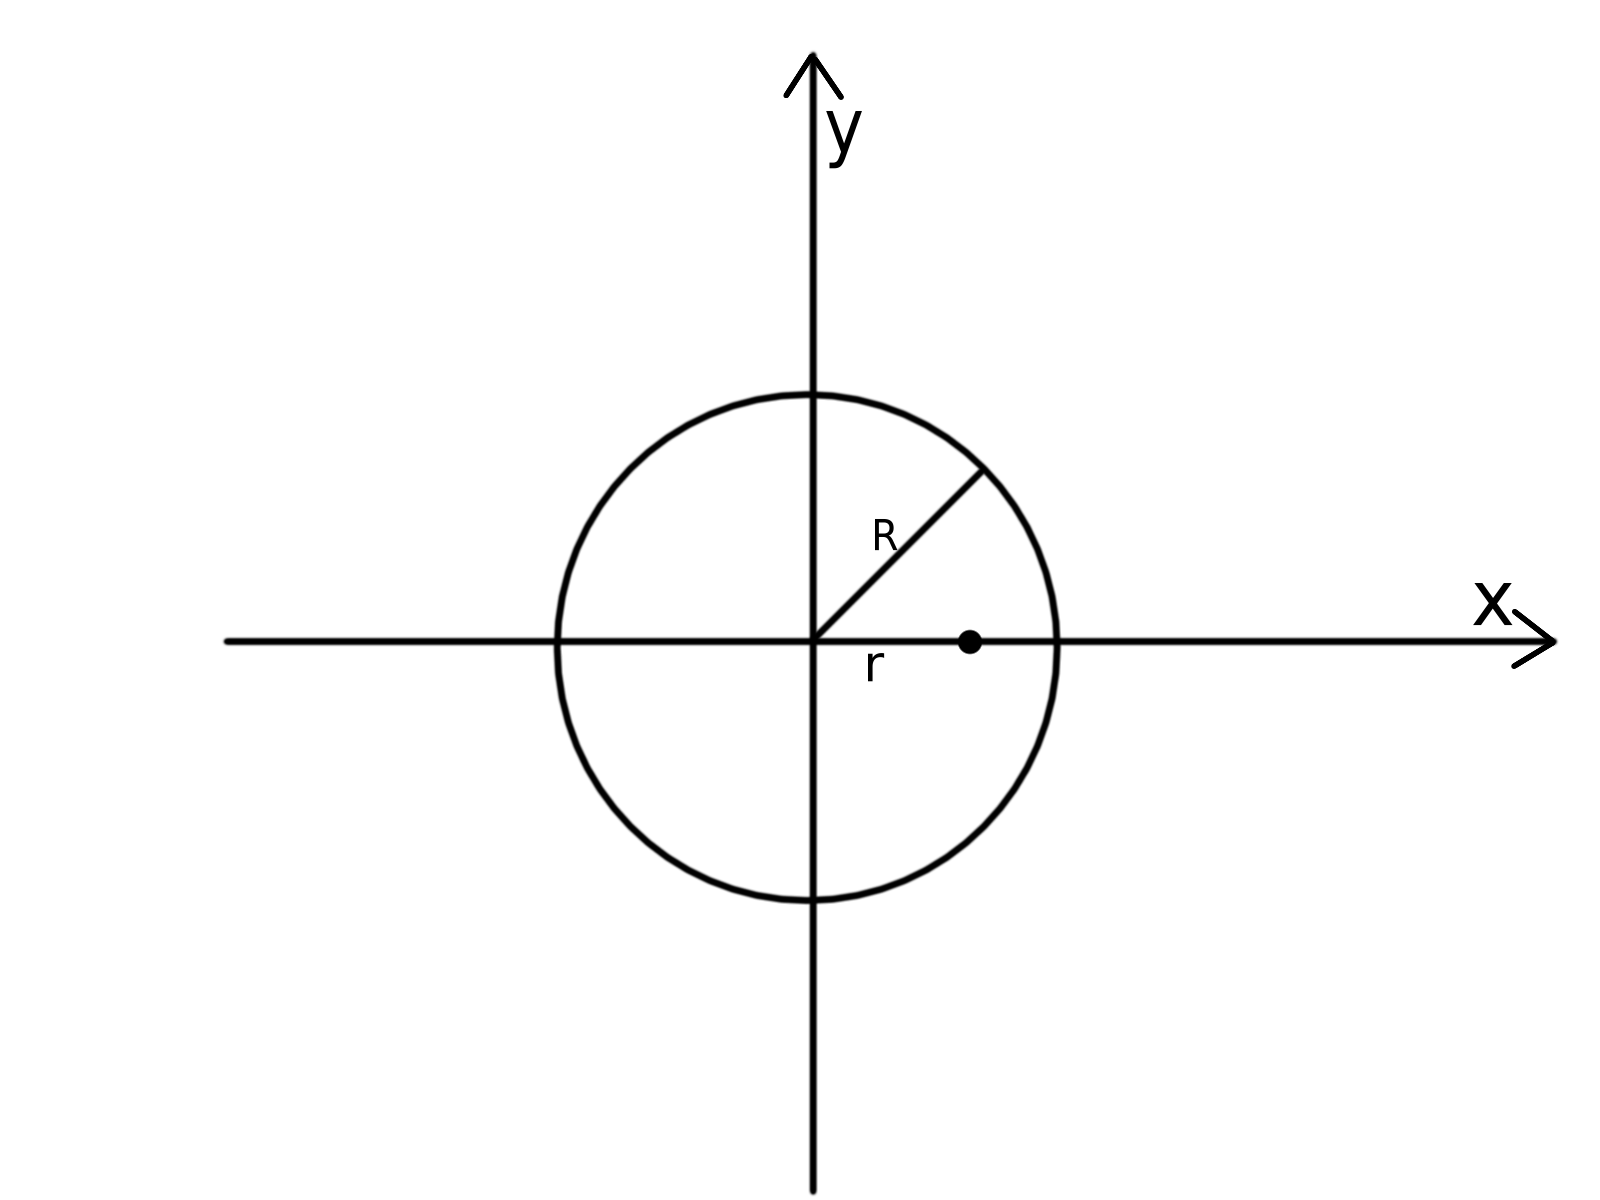
\includegraphics[width=\textwidth]{fig2}
\caption{Figure A}
\end{minipage}
\hfill
\begin{minipage}[b]{0.4\textwidth}
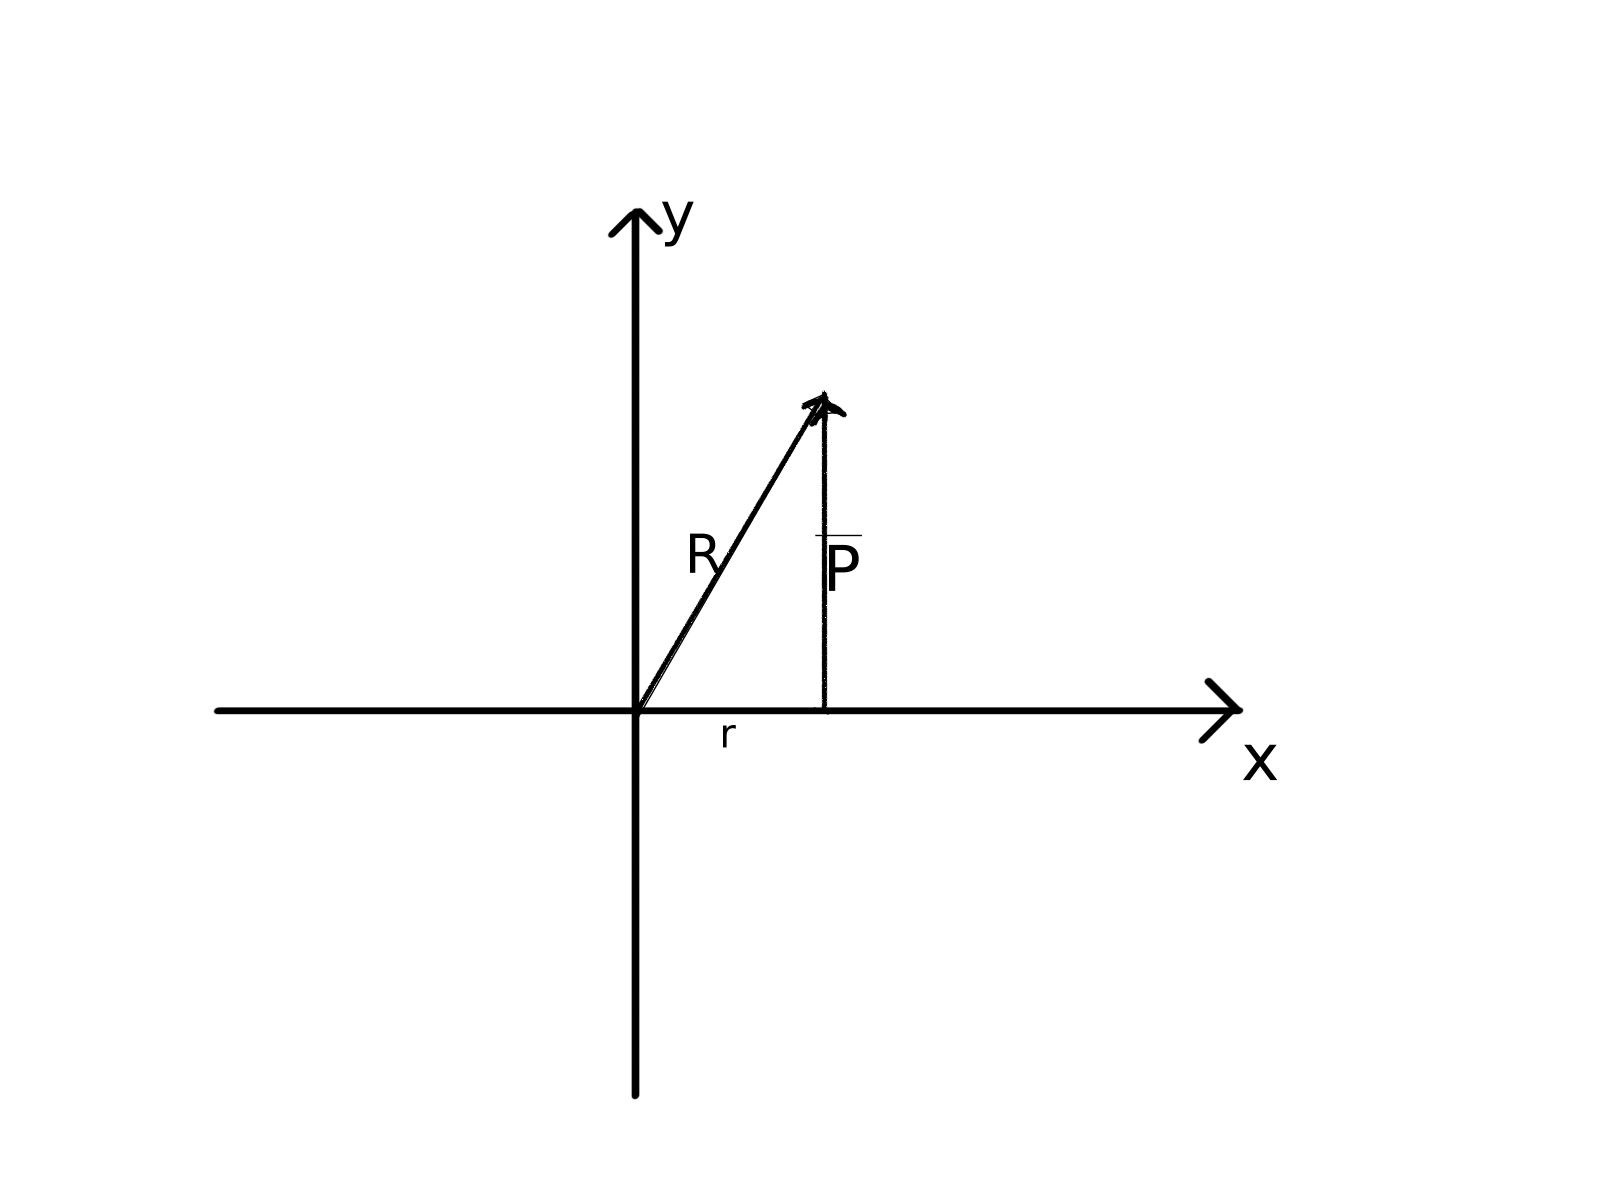
\includegraphics[width=\textwidth]{fig1}
\caption{Figure B}
\end{minipage}
\end{figure}

From Figure (2.5), 

\begin{center}
$ \vec{r} = r.\hat{i} $

$ \vec{R} = R(cos \theta \hat{i} + sin \theta \hat{j} ) $

$ \vec{p} = \vec{R}-\vec{r} $

$ = (R cos \theta-r) \hat{i} + R sin \theta \hat{j} $


$ \vert \vec{p}\vert = \sqrt{(R cos \theta - r)^{2} + (R sin \theta )^{2} }$


 

The Gravitational Potential is given by 

\begin{equation}
 d{\Phi}= \frac{GmdM}{\vert (\vec{p})\vert} 
\end{equation}


$ \Phi = \int {d{\Phi}} $
  

$ d M = \lambda R d \theta  $

By substituting Linear Mass Distribution ,

\begin{equation}
\Phi= \frac{GMmR}{2\pi R} \int_{0}^{2\pi} \frac {d \theta } {\vert \vec{p} \vert^\frac{1}{2}}
\end{equation}

\begin{equation}
\Phi= \frac{GMm}{2\pi} \int_{0}^{2\pi}  
\frac{d{\theta}}{\sqrt{R^2 - 2 R r \cos \theta + r^2}}
\end{equation}


substitution of the following parameters in the equation (2.8) gives us (2.9)

$ d \theta = 2 d \beta $,
$ \theta = \pi - 2 \beta $,
$ \beta = \frac{\pi - \theta}{2} $

\begin{equation}
\Phi (\vec{r}) = \frac{GMm}{ \pi} \int_{0}^{\frac{\pi}{2}}  \frac{d \beta }{\sqrt{r^2 + R^2 +2 R r (1 - 2 \sin^2 \beta )}}  
\end{equation}

\begin{equation}
\Phi (\vec{r}) = \frac{GMm}{ \pi} \frac{1}{\sqrt{q}} \int_{0}^{\frac{ \pi}{2}} \frac{d \beta }{\sqrt{1 - \frac{4 r R}{q} \sin^2 \beta}}   
\end{equation}
 

$ q = r^2 + R^2 +2 r R, $ 
$ k = \sqrt{\frac{4 r R }{q}} $
$ k^2 = \frac{4 r R}{q} $

subtitution of the following in equation(2.10) results in :

\begin{equation}
\Phi (\vec{r}) = \frac{GMm}{ \pi} \frac{1}{\sqrt{q}} \int_{0}^{\frac{ \pi}{2}} \frac{d \beta } {1 - k^2 \sin \beta } 
\end{equation}

we know that the equation 2.12 is the Elliptic Integral of First kind,
\begin{equation}
\frac{d \beta } {1 - k^2 \sin \beta } = K (k) 
\end{equation}
 
by substituting in equation (2.11)

\begin{equation}
 \Phi (\vec{r}) = \frac{GMm}{ \pi} \frac{1}{\sqrt{q}} K (k) 
\end{equation}

Force is given by
\begin{equation}
 \vec{F} = - \bigtriangledown  \Phi 
\end{equation}
\end{center}

we know that,
\begin{center}

\begin{equation}
\frac{\partial K (k)}{\partial k } = \frac{E(k)- (1-k^2) K(k)}{k(1- k^2)} 
\end{equation}
\end{center}
where, E(k) is the Eliiptic Integral of Second kind,

\begin{center}

\begin{equation}
 \frac{\partial q}{\partial r} = 2 (r + R)
\end{equation}

\begin{equation}
 \frac{\partial k}{\partial r} = \frac{2R - k^2 (r + R)}{kq} 
\end{equation}

\begin{equation}
\frac{d K(k)}{d k} = \frac{E(k) - (1-k^2) K(k)}{k (1-k^2)} 
\end{equation}

\begin{equation}
\frac{\partial K (r)}{\partial r} = \frac{d K(k)}{dk} \frac{\partial k }{r} 
\end{equation}

\begin{equation}
\frac{\partial \Phi}{\partial r} = - \frac{GMm }{\pi} [ \frac{E(k) - (1-k^2) K(k)}{k (1-k^2)} (\frac{2R - k^2 (r + R)}{kq} \sqrt{q}) - (\frac{\frac{1}{2} \frac{1}{\sqrt{q}}2 (r + R ) K(k)} {q}] 
\end{equation}

\end{center}

Simplifying,

\begin{center}


$ = - \frac{GMm }{\pi} [\frac{\frac{(E(k)- (1 - k^2 )K(k))(2 R - k^2 (r + R)) - (r + R) K(k) k^2 (1 - k^2)}{k^2 (1-k^2)\sqrt{q}}}{q}] $


$ = - \frac{GMm }{\pi} [\frac{2 R E(k) - E (k) k^2 (r+R) - 2 R(1-k^2) K(k)}{k^2 (1 - k^2) q^\frac{3}{2}}] $





\begin{equation}
 = - GMm \frac{1}{\pi k^2 (1 - k ^2)  q^\frac{3}{2}} [2 R E (k) - k^2 r E(k)- k^2 R E(k) - 2 R K(k) + 2 R k^2 K(k)]
\end{equation}

\begin{equation}
 = - GMm \frac{1}{\pi k^2 (1 - k ^2)  q^\frac{3}{2}} [E (k) 2R - k^2 (r + R) - 2 R K(k) (1 - k^2) ] 
\end{equation}
\end{center}
 
substituting,
 \begin{center}
 $ \mu = k^2  $
 \end{center}


The final expression for Gravitational Force is:
\begin{center}

\begin{equation}
 \vec{F}_{r} = - GMm \frac{1}{\pi q^ \frac{3}{2} (1- \mu)} \frac{1}{\mu} (2 R K(\sqrt{\mu}) (1 - \mu))- E (\sqrt{\mu}) (2 R - \mu (r + R))
\end{equation}

\end{center}

\subsection{Data from Histogram}
To calculate force, we require information about the masses of the rings. For that purpose, we extracted data from the Histogram of masses plotted as a function of normalized intensity. In astronomy, we have direct relation between the Luminosity and Masses of a celestial object, i.e. 

\begin{equation}
\frac{L}{L_{\odot}} = (\frac{M}{M_{\odot}})^4 
\end{equation}

So by saving the values of luminosity from the same file, we used in section 2.2.2 , and convert it into mass using the equation above. 

\subsection{Function Definition for Data Extraction from Histogram}
\begin{verbatim}

    with open('data.csv', 'w') as fout:

        for x in range(w):
            for y in range (h):

                r= calc_distance(x0,y0,x,y)
                i = calc_gs_intensity( andro[x,y] )
                m= i**0.25 

                print (r,i,m)


                fout.write(str(r) + "," + str(i)+ "," + str(m) + "\n")

\end{verbatim}


\subsection{Function Definition for Calculation of Force}
\begin{verbatim}
def q(r,R) :

    return r*r+R*R+2*r*R

def k(r,R,con) :
    b = float(4*r*R)
    return (b/con)

def f(m,M,R,r,con,ks,g):
    d= 2*R - ks * (r+R)
    E=  ellipe(ks**0.5 )          ##(elliptic function of 2nd kind)
    j= (1-ks)
    G= 2*R* ellipk(ks**0.5)       ## elliptic function of 1st kind
    h= math.pi * (con ** 1.5) *j

    return (((-1*M*ms*g)/ h) * (1/ks)* (G *j -E *d) )

def F(ms,M,R,r):

    # print(r)s
    # print(R)
    con = q(r,R)
    # print (con)
    ks = k(r,R,con)
    # print (ks)
    g = 6.67e-11

    # fa = f(m,M,R,r,con,ks,g)
    # print (fa)


    return f(ms,M,R,r,con,ks,g)

\end{verbatim}

\begin{figure}[h]
\centering
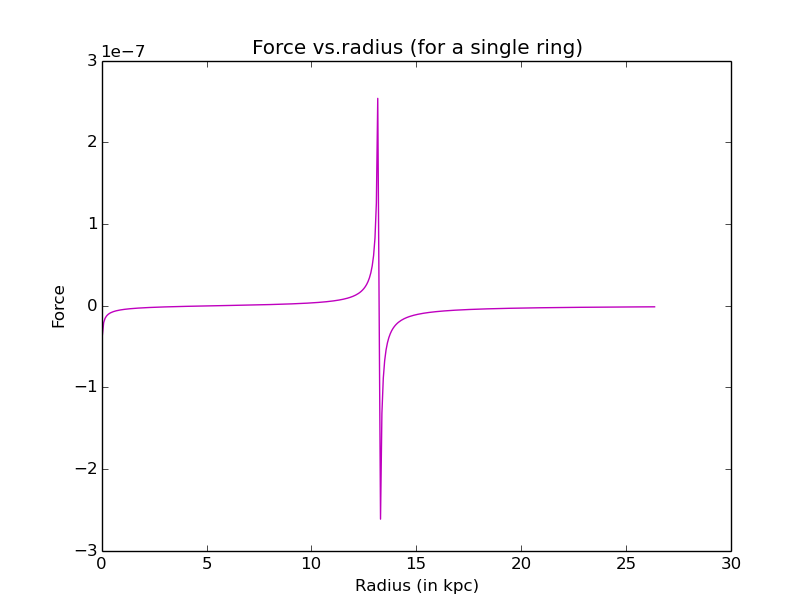
\includegraphics[scale=0.5]{force41R} 
\caption{force on a single ring }
\end{figure}



\section{Calculation for Velocity }

Centripetal force is known to be,

\begin{center}
\begin{equation}
\vec{F_{c} = \frac{m v^2 }{r}}
\end{equation}

\begin{equation}
\vec{F}_{r} = - GMm \frac{1}{\pi q^ \frac{3}{2} (1- \mu)} \frac{1}{\mu} (2 R K(\sqrt{\mu}) (1 - \mu))- E (\sqrt{\mu}) (2 R - \mu (r + R))
\end{equation}

\begin{equation}
v = \sqrt{\frac{GMm \frac{1}{\pi q^ \frac{3}{2} (1- \mu)} \frac{1}{\mu} (2 R K(\sqrt{\mu}) (1 - \mu))- E (\sqrt{\mu}) (2 R - \mu (r + R))}{r}}
\end{equation}

\end{center}

\subsubsection{Function Definition for Velocity}
\begin{verbatim}
 def v(self, rs, v0, m0):

        vs=[]

        self.Mass[0] = m0

        for r in rs:

            T=0

            for i in range(len(self.Rad)):
                R= self.Rad[i]
                M= self.Mass[i]
                if abs(R-r) > 0.5:
                    lF = F(ms,M,R,r)
                    T= T+lF

            v = v0 * (abs(T*r))**0.5
            vs.append(v)

        return vs
\end{verbatim}

\section{Observed Rotation Curve}


The survey of Andromeda Galaxy according to [15], gives us the rotation curve measured out to $38$ kpc, showing a nuclear peak at $340$ km s$^{-1}$ , a dip at $202$ km s$^{-1}$ around $4$ kpc, two distinct flat parts at $264$ km s$^{-1}$  and $230$ km s$^{-1}$ and an increase to $275$  km s $^{-1}$ in the outermost regions.
 
 Regenerating the curve, using the following program,  
\begin{verbatim}

x= []
y= []

with open ('rd.txt','r') as f:
    for row in f:

        x.append((row))



with open ('vrot.txt', 'r') as f1:
    for row1 in f1:

        y.append((row1))


pylab.ylim([0,400])
pylab.xlim([0,35])
plt.plot(x,y)
plt.scatter(x,y)


\end{verbatim}

The following curve is obtained, as the observed rotation curve of M31.

\begin{figure} [h]
\centering
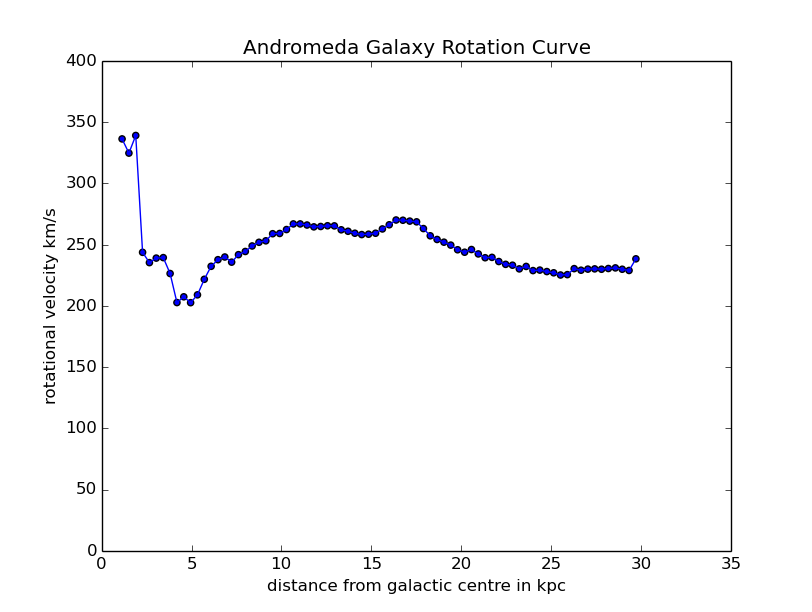
\includegraphics[scale=0.5]{rotcurve}
\caption{Observed Rotation Curve for Andromeda Galaxy}
\end{figure}
\section{Optimization of Velocity and Mass}
The rotation curve obtained from the data, that was calculated using Image Analysis as explained in section 2.2.1  

\begin{verbatim}
a,b = scipy.optimize.curve_fit(fit.v, R, V)
    print (a)
    print b


    v0 = a[0]
    m0 = a[1]
    v = fit.v(R,v0,m0)   #for black hole mass
    pmv = plt.scatter(R,v, color= 'g',label ='m0 & v0')
    plt.plot(R,v)


    vo = fit.v(R,v0,m0_o)  #for very small mass .. i.e the first entry in the list.
    pv = plt.scatter(R,vo , color='y', label = 'v0')
    plt.plot(R,vo)
\end{verbatim}

\begin{figure} [h]
\centering
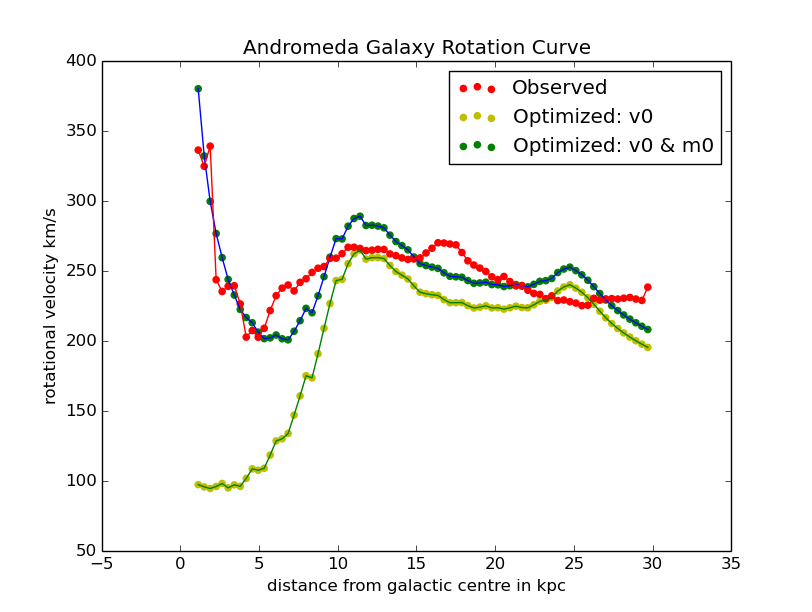
\includegraphics[scale=0.5]{best}
\caption{Rotation Curve for Andromeda Galaxy}
\end{figure}

\section{Need for Optimization}








    	\chapter{Results and discussion}

The survey of Andromeda Galaxy according to [15] gives us the rotation curve measured out to $38$ kpc, showing a peak at $340$ km s$^{-1}$, a dip at $202$ km s$^{-1}$ around $4$ kpc, two distinct flat parts at $264$ km s$^{-1}$  and $230$ km s$^{-1}$ and an increase to $275$  km s $^{-1}$ in the outermost regions \cite{observed}.
\begin{figure} [h]
\centering
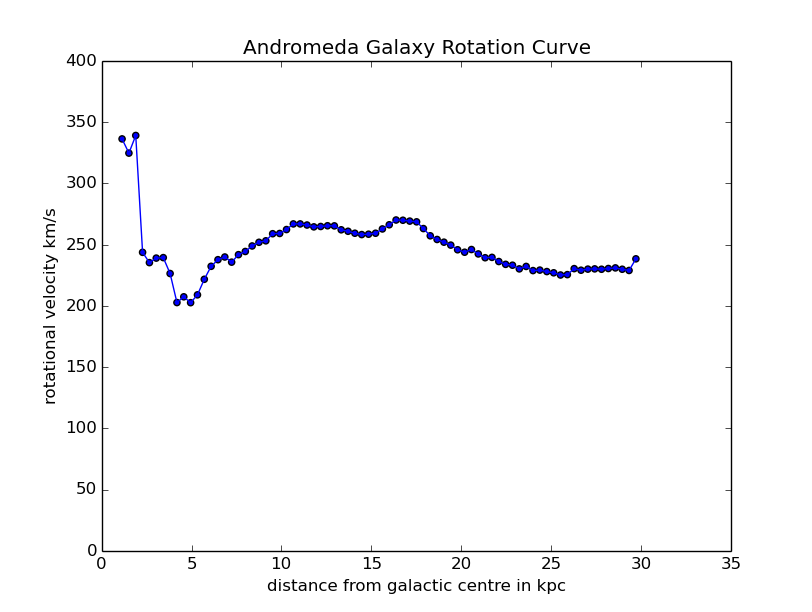
\includegraphics[scale=0.5]{rotcurve}
\caption{Observed Rotation Curve for Andromeda Galaxy}
\end{figure}

\section{Optimized Rotation Curve}

The rotation curve obtained from the data, that was calculated using Image Analysis as explained in section 2.2.1  was optimized, and the resulting plot is:

\begin{figure} [h]
\centering
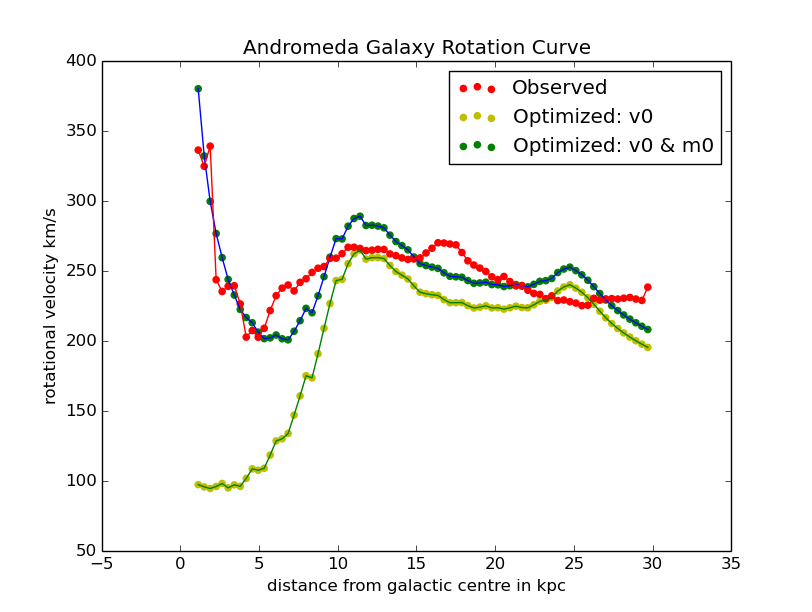
\includegraphics[scale=0.5]{best}
\caption{Rotation Curve for Andromeda Galaxy}
\label{curves}
\end{figure}

\section{Need for Optimization}

The rotation curve obtained by using the precalculated data, was to be achieved by the data calculated using image analysis. When we plotted the curve from our calculated data, it gave us an irregular pattern, which demanded that some fitting be done. After we optimized the graph to a certain velocity the optimization function gave us the fitted value of $v_0$ . From Figure \ref{curves} we found the curve described as \textit{optimized for velocity} \textbf{$v_{0}$} to be somewhat in accordance with the observed rotation curve, but it still required significant modification in the region near the origin.
To that end we optimized the curve for central mass and consequently the function gave us optimized value of \textbf{$m_{0}$}. 

The values of $v_{0}$ and $m_{0}$ were calculated to be;

$v_{0} = 55802.2453 $         

$m_{0} = 1473818.3329 $

with standard deviations of:

$\triangle v =  683.96$

$\triangle m = 88311.38 $

$v_0$ being a scaling factor is dimensionless while $m_0$ is measured in the same arbitrary units as the masses calculated using image analysis. To make sense of $m_0$ note that it is $16%$ of the total calculated mass of the galaxy.
    \chapter{Summary and Conclusion}

Andromeda Galaxy is our nearest neighbour, a spiral galaxy just like the Milky Way, located at about $744$ kpc. This thesis provides a technique to analyze astronomical data and use it to reproduce the rotation curve of Andromeda Galaxy. From Section $3.1$ we saw that the graph optimized only  for velocity shows disagreement with the observed curve, near the centre of the galaxy. When the same graph is optimized for mass, it is quite similar to the one obtained from observed data. We can conclude from this observation that a highly massive body is required at the centre of the galaxy to provide such a high velocity to the bodies in it. This indicates the presence of a super massive black hole at the centre of the galaxy. 

The rotation curve can be further optimized by incorporating the MOND parameter $a_0$. This will be the focus of future work.
    \chapter{Code}
\section{Calculation of Distances and Intensity}
\begin{verbatim}
import matplotlib.pyplot as plt
import csv
import matplotlib.mlab as mlab
import numpy as np



import math
from scipy import misc
# np.seterr(over='ignore')


x0 = 88.23
y0 =1675.78

denom= math.sqrt(3)*255

def main():


    andro = misc.imread('andromeda.jpg')
    (w, h,d) = andro.shape



    with open('data.csv', 'w') as fout:

        for x in range(w):
            for y in range (h):

                r= calc_distance(x0,y0,x,y)
                i = calc_gs_intensity( andro[x,y] )
                m= i**0.25

                print (r,i,m)


                fout.write(str(r) + "," + str(i)+ "," + str(m) + "\n")





# i: numpy.ndarray with 3 values: R, G, B
# This function takes the array and converts from RGB to greyscale intensity value between 0 and 1
denom= math.sqrt(3)*255

def calc_gs_intensity(i):


    R = float(i[0])
    G = float(i[1])
    B = float(i[2])

    return math.sqrt(R*R+G*G+B*B)/denom


def calc_distance(x0,y0,x,y):

    x_dist = (x - x0)
    y_dist = (y-y0)

    return  math.sqrt(x_dist*x_dist+y_dist*y_dist)


if __name__ == '__main__':
    main()
\end{verbatim}

\section{Histogram for 400 Bins}
\begin{verbatim}
import csv
import matplotlib.pyplot as plt


def main():

    reader = csv.reader (open('data.csv', 'rb'), delimiter=',')

    R = []
    m= []

    for row in reader:
        r= float(row[0])
        #print r
        R.append( r* 0.005620)
        m.append( float(row[2]) )

    plt.hist(R, weights=m, bins = 400)
    n,bins,patches = plt.hist(R, weights=m, bins = 400) ## gets the value of bin boundaries and weights for each bin ..
    #print(n)
    #print (bins)

    with open('histdata.csv', 'w') as fout:

        for i in range(len(n)):
            fout.write(  str((bins[i] + bins[i+1])/ 2)+ ", " +str(n[i]) + "\n") ##calculates the midpoint of each bin and saves it to file. + saves the value of weights for each bin

    plt.title('Mass distribution of Andromeda')
    plt.xlabel('radius   (Kpc)    1pixel = 0.05620 kpc<  ')
    plt.ylabel('Masses relative to intensity')
    plt.show()




if __name__ == '__main__':

    main()
\end{verbatim}

\section{Observed Rotation Curve}
\begin{verbatim}
import numpy as np
import matplotlib.pyplot as plt
import pylab



x= []
y= []

with open ('rd.txt','r') as f:
    for row in f:

        x.append((row))



with open ('vrot.txt', 'r') as f1:
    for row1 in f1:

        y.append((row1))


pylab.ylim([0,400])
pylab.xlim([0,35])
plt.plot(x,y)
plt.scatter(x,y)


plt.title ('Andromeda Galaxy Rotation Curve')
plt.xlabel('distance from galactic centre in kpc')
plt.ylabel('rotational velocity km/s')
plt.show()
savefig('plot.jpg')

\end{verbatim}

\section{Force and Velocity Calculation and Optimization}
\begin{verbatim}
import csv
import numpy as np
import scipy
from scipy.special import ellipk, ellipe
import matplotlib.pyplot as plt
from pylab import *
import matplotlib.pyplot as plt
import pylab
from scipy.optimize import curve_fit
from numpy import array
import numpy

g = 6.67e-11
ms=1  #mass of the point
numpy.seterr('raise')

def main():

    Mass =[] #mass of the ring
    Rad=[]

    with open ('histdata.csv', 'r') as f:
        for row in f:
            values= row.split(',')

            Rad.append(float(values[0])) #saves values of radius from data file in empty list.
            Mass.append(float(values[1]))

    m0_o = Mass[0]

    # plt.plot(Rad,Mass)
    # plt.show()

    fit = Fit(Rad, Mass)

    x= []
    y= []

    with open ('rd.txt','r') as f:
        for row in f:

            x.append(float(row))



    with open ('vrot.txt', 'r') as f1:
        for row1 in f1:

            y.append(float(row1))



    R = numpy.array(x)
    V = numpy.array(y)

    #
    a,b = scipy.optimize.curve_fit(fit.v, R, V)
    print (a)
    print b


    v0 = a[0]
    m0 = a[1]
    v = fit.v(R,v0,m0)   #for black hole mass
    pmv = plt.scatter(R,v, color= 'g',label ='m0 & v0')
    plt.plot(R,v)


    vo = fit.v(R,v0,m0_o)  #for very small mass .. i.e the first entry in the list.
    pv = plt.scatter(R,vo , color='y', label = 'v0')
    plt.plot(R,vo)


    # a,b = scipy.optimize.curve_fit(fit.vn, R, V)   #optimizing without the mass.. only velocity will give a large value.
    # print (a,b)
    #
    # v0= a[0]
    #
    #
    # vm = fit.vn(R,v0)
    # plt.scatter(R,vm, color= 'c')
    # plt.plot(R,vm, color= 'c')

    # a,b = scipy.optimize.curve_fit(fit.K, R, V, None, None, False, True, ([1, 0, 1],[np.inf, np.inf, 1.5]))
    #
    # v0= a[0]
    # m0 = a[1]
    # km = a[2]
    #
    # kc = fit.K(R,v0,m0,km)
    # plt.scatter(R,kc, color= 'm')
    # plt.plot(R,kc, color= 'm')
    # print (v0,m0,km)

    # a,b = scipy.optimize.curve_fit(fit.v_mond, R, V)
    # print ('v_mond gives: \n')
    # print (a)
    # print b


    # v0 = a[0]
    # m0 = a[1]
    # a0 = a[2]
    # v_m = fit.v_mond(R, v0,m0,a0)
    # plt.scatter(R,v_m, color= 'c')
    # plt.plot(R,v_m, color= 'c')


    curve= velocity_curve(Rad,Mass)

    # po= act_curve(x,y)
    # plt.legend([po,pv,pmv ], ['Observed', 'Optimized: v0','Optimized: v0 & m0 ' ])
    plt.show()

def act_curve(x,y):

    # x = x[:100]
    # y = y[:100]


    # pylab.ylim([0,400])
    # pylab.xlim([0,35])
    plt.plot(x,y, label = 'Observed')
    po= plt.scatter(x,y, color ='r')



    plt.title ('Andromeda Galaxy Rotation Curve')
    plt.xlabel('distance from galactic centre in kpc ')
    plt.ylabel('rotational velocity km/s')
    # plt.show()
    return po



def velocity_curve(Rad, Mass):

    force = []
    vel = []
    j=200

    for r in Rad:       ##for force inside the point we want to calculate, r will be fixed and R will be changing.
        T=0

        for i in range(len(Rad)):
            R= Rad[i]
            M= Mass[i] if i == j else 0
            if  r!=R:
                lF = F(ms,M,R,r)
                # print(lF,r,R,M)
                T= T+lF

        force.append(T)

        print(r,T)
    # print(len(force))
    # print (len(Rad))
    print (F(ms,10,13,0.001))


    plt.plot(Rad,force, color = 'm')
    plt.title('Force vs.radius (for a single ring)')
    plt.xlabel('Radius (in kpc)')
    plt.ylabel('Force')


    # for j in range(len(Rad)):
    #     r=Rad[j]
    #     f= force[j]
    #     v= ((-f*r)/ms)**0.5
    #     # print (r,f,v)
    #     vel.append(v)
    # plt.plot(Rad,vel)
    # plt.scatter(Rad,vel, color = 'c')
    # plt.title('Velocity vs Radius')
    # plt.xlabel('Radius (in parsecs)')
    # plt.ylabel('velocity')

    plt.show()

def q(r,R) :

    return r*r+R*R+2*r*R

def k(r,R,con) :
    b = float(4*r*R)
    return (b/con)

def f(m,M,R,r,con,ks,g):
    d= 2*R - ks * (r+R)
    E=  ellipe(ks**0.5 )##(elliptic function of 2nd kind)
    j= (1-ks)
    G= 2*R* ellipk(ks**0.5) ## elliptic function of 1st kind
    h= math.pi * (con ** 1.5) *j

    return (((-1*M*ms*g)/ h) * (1/ks)* (G *j -E *d) )

def F(ms,M,R,r):

    # print(r)s
    # print(R)
    con = q(r,R)
    # print (con)
    ks = k(r,R,con)
    # print (ks)
    g = 6.67e-11

    # fa = f(m,M,R,r,con,ks,g)
    # print (fa)


    return f(ms,M,R,r,con,ks,g)


class Fit:

    def __init__(self, Rad, Mass):

        self.Rad = Rad
        self.Mass = Mass


    def v(self, rs, v0, m0):

        vs=[]

        self.Mass[0] = m0

        for r in rs:

            T=0

            for i in range(len(self.Rad)):
                R= self.Rad[i]
                M= self.Mass[i]
                if abs(R-r) > 0.5:
                    lF = F(ms,M,R,r)
                    T= T+lF

            v = v0 * (abs(T*r))**0.5
            vs.append(v)

        return vs

    def vn(self, rs, v0):

        vs=[]

        for r in rs:

            T=0

            for i in range(len(self.Rad)):
                R= self.Rad[i]
                M= self.Mass[i]
                if abs(R-r) > 0.5:
                    lF = F(ms,M,R,r)
                    T= T+lF

            v = v0 * (abs(T*r))**0.5
            vs.append(v)

        return vs

    def K(self, rs, v0,m0, km):  #any optimizing constant ... now not required.

        vs=[]
        self.Mass[0] = m0

        for r in rs:

            T=0

            for i in range(len(self.Rad)):
                R= self.Rad[i]
                M= self.Mass[i]*km
                if abs(R-r) > 0.5:
                    lF = F(ms,M,R,r)
                    T= T+lF

            v = v0 * (abs(T*r))**0.5
            vs.append(v)

        return vs

    def v_mond(self, rs, v0,m0,a0):  #fitting for mond .. which didnt work..

        vs=[]

        for r in rs:

            T=0

            for i in range(len(self.Rad)):
                R= self.Rad[i]
                M= self.Mass[i]
                if abs(R-r) > 0.5:
                    lF = F(ms,M,R,r)
                    T= T+lF


            v = v0 * ((a0/((ms*a0)-T))*abs(T*r))**0.5
            vs.append(v)

        return vs


if __name__ == '__main__':
    main()




\end{verbatim}
 

    \makereferences         % Create the references section

\end{document}
